
\section{Implementation}

We provide details about the nearest neighbor computation with Patch Match~\cite{Barnes09} and its multiple exemplar version, borrowing ideas from Patch Web~\cite{Barnes11}. We present our patch selection using GIST.
Finally, we mention details about the different transfer strategies and discuss the frame disparity computation.

Along this section, we assume that the input frame $L'$ is the left frame and we find a k-NNF from its patches to patches within the left images $L$ of our database.
The database also contains the corresponding right frames $R$ and our goal is to eventually synthesize $R'$ from $L'$.

We assume our images to have $4$ channels: the usual $L+a+b$ from CIELAB that provide perceptually-motivated L2 distances, as well as an extra $y$ channel that encodes the location of pixels within the image, which accounts for disparity being usually larger at the bottom of images than at the top (this helps convergence).
All the channels are normalized to be within $[0;1]$.


\subsection{Patch Match}

Given an input image $A$ made of overlapping $N\times N$ patches $\{\ti\}$, we want to find the closest patches $\{\si\}$ in an image $B$, i.e.
\begin{equation}
	\si^{*} = \argmin_{\si \in B} d(\ti, \si)
\end{equation}
for some distance $d(\cdot)$, usually the sum of squared differences or a L2 norm.

A naive brute-force computation would enumerate all possible patch assignments and find the best one.
However, this is computationally unreasonnable given the context of our large high resolution image database.

Patch Match~\cite{Barnes09} is a fast approximate nearest neighbor algorithm specifically tuned for image patches and thus our problem.
It is based on the \emph{coherence assumption}, namely that, while patches mapped from $A$ to $B$ can be mapped everywhere in $B$, nearby patches in $A$ are usually mapped together in $B$.

\begin{figure}[ht]
\centering
	\begin{subfigure}[t]{0.155\textwidth}
		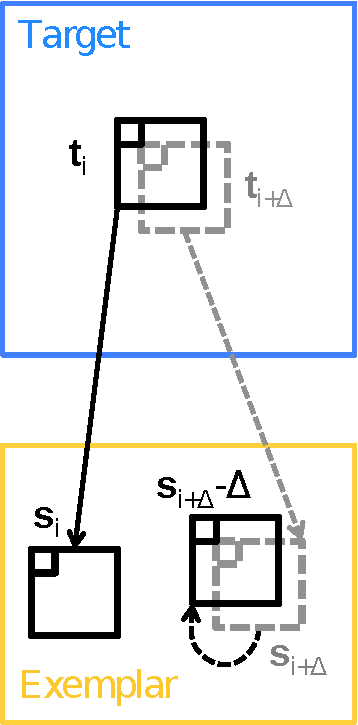
\includegraphics[width=\textwidth]{figures/propagation_text2}
		\caption{Propagation}
	\end{subfigure}
	\begin{subfigure}[t]{0.155\textwidth}
		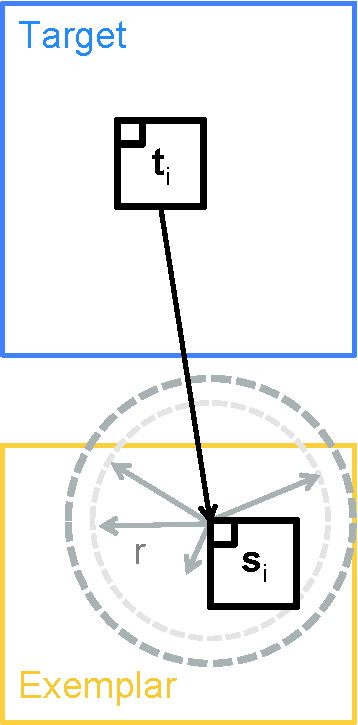
\includegraphics[width=\textwidth]{figures/randsearch_text}
		\caption{Random search}
	\end{subfigure}
	\begin{subfigure}[t]{0.155\textwidth}
		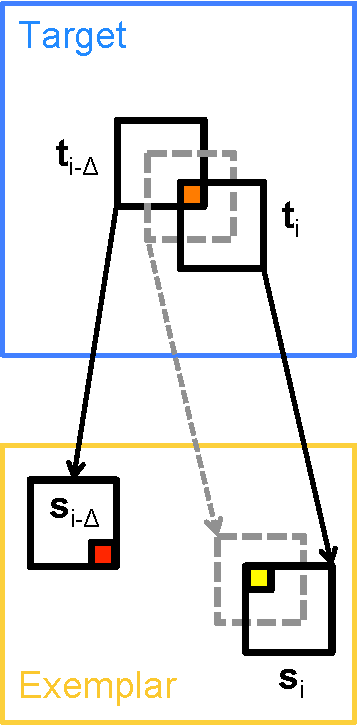
\includegraphics[width=\textwidth]{figures/voting_text}
		\caption{Voting}
	\end{subfigure}
   \caption{The main components of texture synthesis using Patch Match.}
\label{fig:texsynth_patchmatch}
\end{figure}

The algorithm proceeds in scanline-order from an initial guess of the nearest neighbor assignments $\{\ti \to \si\}$ and tries new candidate nearest neighbor patches using two main operations:
\textbf{propagation} which tries to propagate the result of neighboring mappings, and 
\textbf{random search} that randomly samples patches in an exponentially decreasing window (see illustrations in Figure~\ref{fig:texsynth_patchmatch}).

Given these patch assignments, we can transfer localized data.
This last step involves different strategies which we details in Section~\ref{sec:transfer}. 
All of them are forms of \emph{voting} since by having $N\times N$ patches, each of the pixels of our output image technically has as many overlapping patches to choose from.
The usual voting consist of averaging the overlapping pixels which minimizes the average L2 distance.

\paragraph{Extensions}
The Patch Match algorithm has been extended in several ways \cite{Barnes10} including the sampling of rotations, scales and mirrored patch spaces, the use of gain and bias adjustment, a $k$-NN version of the algorithm as well as extra operations (uniform sampling, enrichment and binning).

Application-specific variants of voting have been explored such as Meanshift \cite{Wexler07}, Histogram weighting \cite{Kopf07} as well as Bidirectional Similarity \cite{Simakov08}.

\subsection{Patch Web}
Extending the algorithm to multiple exemplars can seem straightforward: patches now also contain new variable index which represents the exemplar they come from.
However, in practice, dealing with multiple images (and potentially many of them) involves dealing with caching and distributing the computation wisely.

\subsubsection{Additional sampling strategies}
To improve performance, the original algorithm~\cite{Barnes11} makes use of three additional sampling strategies:

\paragraph{Uniform sampling} searches over all patches of all exemplars (this is very similar to random search, with a new exemplar dimension to search through).

\paragraph{Enrichment} finds new candidates by looking at what patches we are mapped to, are mapped to (forward enrichment $f$) or to use the reverse mapping (backward enrichment $f^{-1}$) similarly.
Variants consider multiple hops such as $f^2$, $f^3$, $\dots$ or $f^{-2}$, etc.

Given a $k$-NNF, one can use enrichment with the $k$ candidates or a subset, leading to many potential variants.

\paragraph{Binning} divides the patches into bins similarly as with a histogram, and samples patches from the bin corresponding to the patch we sample for.
To bin patches, usually a lower-dimension space is used ($N\times N$ patches with $C$ channels have $CN^2$ dimensions) by computing PCA.

Recent alternatives~\cite{He12} use Walsh-Hadamard Transform bases~\cite{Hel05} instead of PCA.

Our implementation contains all the aforementioned candidate lookups but binning because of the high memory requirement that makes it harder to implement wisely (other strategies require basically no additional memory storage).
Note that WHT is a better candidate than PCA because it can be computed with much fewer operations (and thus a cache-friendly strategy using it can be envisioned).

\subsubsection{Computing the web}
The general idea is to computer the $k$-NNF from one image in the web to a group of other images and repeat until the web is good enough.
In an ideal world, all images could be loaded at the same time, but given the context of large high resolution images we target, this is not possible.
Instead, we must iteratively do in parallel (for different instances $i$):
\begin{enumerate}
	\item Compute the $k$-NNF from $A_i$ to a subset $\mathbf{A}_i$
	\[ 
		\mathbf{A}_i \subset \bigcup_{j\neq i}{A_j}
	\]
	\item Potentially merge the resulting $k$-NNF with other parallel $k$-NNFs (use minimum distance mappings)
	\item Store/load data on/from disk
	\item Have data caching to compute distances to patches which are not in our current image set\footnote{Otherwise, one must constrain the individual NNFs to always have patches from images in their current lookup set $\mathbf{A}_i$ which is a strong restriction}
\end{enumerate}

\paragraph{Image Subset} we have to eventually process each image once, and to maximize mixing, we start by grouping patches into similar batches, which we compute using GIST features.
Given an image $A_i$ and a budget of $M$ images, for a heterogeneous dataset (not successive similar images), we group $A_i$ with images that have similar GIST descriptors.
We keep a table of the groups and don't process a same group twice since the distance can only get smaller over time.

\paragraph{Convergence} is determined by looking at the number of effective updates done within a $k$-NNF computation.
If no better patch is found for $A_i$, we can short-circuit its scanline processing and go on with other groups.

For a given image, we declare that its $k$-NNF has converged if its best layer (out of the $k$) has distances below some threshold, or a fixed number of iterations has been reached.
The whole algorithm has converged when each individual $k$-NNF has converged.

Since everything is saved to disk, the process can be stopped and resumed later.

\subsection{Stereo Transfer}
\label{sec:transfer}
Armed with an effective multiple exemplar $k$-NNF computation, there remains to transfer the stereoscopic information and synthesize our right frame.

\paragraph{Patch and difference transfer:} we first reduce the $k$-NNF into a single best-layer NNF, and we then use a simple voting strategy with a $7\times 7$ Gaussian mask ($\sigma=1$) for the weight of each overlapping patch so as to reduce blurring.

\paragraph{Disparity transfer:} we transfer it by simply warping our left image $L'$ according to the disparity between $L$ and $R$..

To compute the disparity of each database pair, we used Classic-NL~\cite{Deqing10} for which a fast and simple Matlab/C++ implementation exists.
We also tried to implement our own disparity computation using Patch Match and it turned out to have a higher resolution. However some results were too noisy to be useful.

\paragraph{Disparity computation with Patch Match} several Patch Match-based methods have appeared in the Middlebury evaluations~\cite{Scharstein02}, with a generally fast runtime and good error evaluations~\cite{Bleyer11, Heise13, Jiangbo13, Besse14}.
Extending our Patch Match implementation to compute disparity is simple, we simply modified our set of candidate proposals with:
\begin{itemize}
	\item \emph{Uniform Horizontal Sampling}: uniform sampling with a horizontal constraint
	\item \emph{Random Horizontal Sampling}: random sampling with a decreasing window, and a horizontal constraint
	\item \emph{Propagation}: as usual (we allow vertical deviation by only a few pixels)
	\item \emph{Random Propagation}: propagates the disparity from a uniformly sampled patch
	\item \emph{Local Mean}: uses the weighted average of samples around the current patch (considering only the one-ring neighborhood gives the best results)
\end{itemize}

Furthermore, we vote the disparity by constraining the maximum motion to the 97.5 percentile of disparities within the resulting image (to remove spurious noise).
While such method is not as smooth and doesn't compare to state-of-the-art disparity computations, it produces higher resolution disparity maps than Classic-NL, for an acceptable running time (only a few tens of seconds for mega-pixel images using a $k$-NNF with $k=7$).